\documentclass{article}

% Language setting
% Replace `english' with e.g. `spanish' to change the document language
\usepackage[english]{babel}

% Set page size and margins
\usepackage[letterpaper,top=2cm,bottom=2cm,left=3cm,right=3cm,marginparwidth=1.75cm]{geometry}
% Useful packages
\usepackage{amsmath}
\usepackage{graphicx}
\usepackage{minted}
\usepackage[colorlinks=true, allcolors=blue]{hyperref}

\title{Homework 2 \\ Language Based Technology for Security} 
\author{Niccolo' Piazzesi \\ n.piazzesi@studenti.unipi.it}

\begin{document}
\maketitle
\frenchspacing

\section*{Introduction}
For this homework, i will present and discuss the paper "\textbf{MirChecker: Detecting Bugs in Rust Programs via Static Analysis}" by 
Zhuohua Li, Jincheng Wang, Mingshen Sun, and John C.S Lui \cite{li2021mirchecker}. This paper present a novel static analysis tool for the Rust programming language, 
focusing on detecting and preventing potential runtime crashes and memory safety bugs.
\section*{Paper Summary}
We can divide the paper in four parts: at the beginning, all the necessary background knowledge about static analysis and Rust 
is established, and the main motivations for the tool development are explained. Then, the high level design of the tool is presented, and the reasoning behind all the relevant choices is 
given. After that, the authors delve deeper in the actual implementation, showing the algorithm used and giving all the important technical details. The last part is about a series of benchmark used to 
test both the efficacy and speed of the developed tool on target examples. Finally, the authors discuss the achieved results, limitations, and the potential future directions of their work.
\subsection*{Background Knowledge and Motivations}
The paper begins by giving the basic knowledge needed to understand its results. The authors start by presenting all the necessary  theory and concepts of abstract interpretation. 
They recall the notions of \textbf{lattice} and \textbf{abstract transfer functions}, showing how they are  used to represent computations on abstract program states. 

In the next part, there is an introduction on the  main features of Rust, mainly about its 
powerful type and ownership system. It is mentioned how the restrictive rules for aliasing and mutability prevents many of the typical memory corruption problems. After, the main motivation for the work is presented: although 
Rust has very advanced tools for memory safety, their incomplete nature and the presence of the \mintinline{rust}{unsafe} keyword  can breach its safety promises, leading  to undetected bugs or worse, undefined behavior. The paper focus on two 
classes of issues affecting the language: \begin{itemize}
    \item \textbf{Runtime panics}.  Rust's type system cannot enforce all the security conditions statically. Some conditions such as array bounds checking or integer overflow detection are postponed until execution, with 
    the compiler automatically instrumenting assertions that, when violated, halt the program. Although this is still a safe way to handle these issues (no memory corruption is possible), an attacker could still exploit this 
    to cause denial of service.
    \item \textbf{Lifetime corruptions.} While  classical memory corruption bugs such as use-after-free or dangling pointers are well managed in Rust, using \mintinline{rust}{unsafe} and combining 
    it with the ownership system may lead to lifetime bugs where, first the unsafe code  causes invalid pointers or shared mutable memory, and then the ownership system automatically drops that memory, leading back to use after free bugs.
\end{itemize}
To prevent these issues, the authors decided to combine numerical static analysis to detect possible runtime panics generated by integer operations,
 and symbolic analysis to track heap memory ownership.
\subsection*{High level design}
MirChecker performs static analysis on top of Rust's Mid-level Intermediate Representation (MIR). MIR is produced as an intermediate step during normal compilation. 
It corresponds to a control flow graph (CFG) representation  and borrow checking is performed on it. Traditionally, Rust static analysis tools reason on LLVM IR or  a custom IR, but the authors decided to use MIR 
for two main reasons. First, while it reduces most of the complex syntax to a simpler core language, it preserves type information and debugging data, which is used to simplify the actual algorithm.
Second, LLVM API targets directly C/C++ and are then ported to Rust. Many compatibility issues may arise, differently from using 
a native representation. 


\paragraph*{User interface} MirChecker is shipped as a subcommand of  
Cargo, Rust's official package manager. This makes it possible to reuse the entire
Rust compiler toolchain for dependency resolving. Dependency information is used 
to distinguish between source files in the current crate (crates are how packages in Rust are called) and dependencies, which are ignored 
by MirChecker for efficiency purposes. Tool invocation is highly customizable, with many options 
to control the behavior of the analysis. Some of the options are shown in \autoref{mir-cli}.
\begin{figure}[H]
\begin{minted}{bash}
    cargo mir-checker --\ 
    --entry <entry-function-name>\
    --domain <abstract-domain>\ 
    --widening_delay <N>\
    --narrowing_iteration <N>\ 
    --suppress_warnings <S>
\end{minted}
    \caption{MirChecker example invocation}
    \label{mir-cli}

\end{figure}


\paragraph*{Static analyzer}
The analyzer is implemented as a custom callback function for the Rust compiler, and is 
automatically called after all the necessary data structures are built. 

The actual algorithm uses standard techniques from Abstract Interpretation.
The CFG is first preprocessed to create a topological ordering of the basic blocks. After, the algorithm traverse the CFG according to the ordering 
and iteratively executes \textit{Abstract Interpretation} until the result reaches a fix-point.
In the following step, several bug detectors are called. These bug detectors use 
constraint solving techniques to determine if some security conditions are violated or not. At the end, a series of 
diagnostics are emitted to the users, leveraging the compiler infrastructure to provide clear and informative messages.
\autoref{fig:hilev} provides a visualization of the entire process.
\begin{figure}[H]
    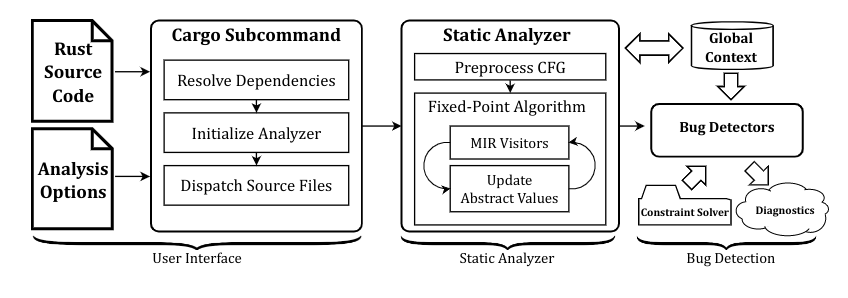
\includegraphics[scale=0.5]{hilev.png}
    \caption{High level view of Mir-Checker architecture}
    \label{fig:hilev}
\end{figure}
\subsection*{Implementation}
\subsection*{Benchmarks}
MirChecker  was thoroughly tested both in precision and efficiency. The evaluation was performed
in two steps. First, it was evaluated in a "supervised" environment, testing its capacity on a synthetic dataset 
containing well known bugs. All the bugs (4 memory safety bugs, 6 runtime panics) where successfully detected. 

In the second phase, 
MirChecker ability was judged in real life situations. A group of actual Rust crates was collected, with the requirement of having related code to 
the tool itself. This meant collecting crates that perform integer arithmetic and/or use unsafe Rust. The results were pretty interesting: the tool managed to find
17 real runtime panics and 16 real memory-safety problems. 

On the bad side, it was noticed that most of the detected problems 
were false positives. Although this is expected in static analysis, in order to have
a more reliable analysis, an option to suppress specific classes of warnings was implemented. It should be mentioned that, even after warning suppression, there were two outliers (the \textbf{brotli} and \textbf{runes} crates) where the rate 
of false positives stayed at 95\%.

\paragraph*{Efficiency} In terms of efficiency, MirChecker was measured both in time and peak memory usage. It was observed that 
the main factor affecting performance is the number of security conditions checked, especially numerical conditions. The choice of the numerical abstract domain 
was found to be the critical tradeoff between efficiency and precision. Interval and linear congruence  consumed less resources but were not as precise as constraint-based domains 
like octagon and polyhedra, which in turn required more memory and time. Another aspect tested was  the dead variable cleaning mechanism 
employed by MirChecker. It was measured to improve performance by 
 10-15\% for constraint-based domains,  while having no major effect for linear congruence and interval domains. 
 
 \section*{Advantages}

 \paragraph*{Cargo integration} I think that integrating a static analysis tool inside a language toolchain is a great idea. 
 Static analysis can benefit a lot from compilation information, as demonstrated by MirChecker dead variable analysis or its 
 informative error messages. Other than that, it favours adoption by end users, who can benefit from the additional checks without 
 having to modify their familiar workflow.


 \paragraph*{Using Z3 for bug detection} The authors decided to use Z3 for the bug detection phase. I think this is a 
 strong point of their work. Z3 is a powerful and industry tested SMT solver, featuring many different theories such as integer 
 arithmetic,bit-vectors, uninterpreted functions and many others. By using this power, MirChecker can detect many bugs by simply 
 converting its internal assertions to a Z3 formula and "outsourcing" the actual solving. Not only does this makes the bug solving more robust, 
 it significantly simplifies MirChecker design, which can be focused on optimizing the fix-point algorithm, instead of having to add a custom internal solver.

\section*{Disadvantages}

\paragraph*{Memory model}
The memory model is, by admission of the authors, lightweight and syntax driven. MirChecker may distinguish 
two  equivalent expressions used as memory addresses simply because the are syntactically different. This makes the analysis 
less precise, and it forced the authors to employ the reduction rules seen before to try and mitigate the issue. The development of an improved
memory model, maybe adapting known formal models  (e.g the concept of heaplets in separation logic), should be a top priority to  
increase the power of the analysis.

\paragraph*{Ignoring Rust advanced features}
For simplicity, MirChecker does not check more advanced features of rust such as dynamic dispatch, concurrent code and many others. While 
this is understandable from a complexity point of view, i think it hinders the analyzer power and convenience. This is true especially for concurrency, 
where problems like deadlocks when using \mintinline{rust}{Mutex<T>} or data races inside unsafe code could be automatically detected.

\section*{Possible Improvements}

\paragraph*{Increasing the number of problems checked}
Right now MirChecker checks only integer operations and possible lifetime issues. 
A first improvement would be to check for more problems. For example, the overflow 
analysis could be extended to floating point operations, which could be extremely valuable 
to analyze math-intensive crates such as \textbf{ndarray} or \textbf{nalgebra}. Another possibility wou

\paragraph*{Refinement}
To mitigate the problem of false positives, the authors could employ a refinement mechanism. Refinement techniques 
takes variou
\paragraph*{Under-approximation instead of over-approximation}

\bibliographystyle{plain}
\bibliography{bib.bib}
\end{document}